% Reports (up to ~2500 words including references, notes and captions–corresponds to ~3 printed pages in the journal) present important new research results of broad significance. Reports should include an abstract, an introductory paragraph, up to four figures or tables, and about 30 references. Materials and Methods should be included in supplementary materials, which should also include information needed to support the paper's conclusions.



\section{Main contributions}

\begin{itemize}
    \item Pattern: Large 2nd/3rd waves, B.1.1.7 dominant variant, steep fall in spring
    \item Many policies and developments at once: Seasonality, NPIs (private / school closures / workplace restrictions), , vaccinations, tests.
    \item Model that makes the most of many available data sources to gauge the relative effects in this transition period -- see joint distribution of infections with age, geography. But contacts with age, geography, occupations.
    \item Intuitive -- directly work with primitives
    \item Very general approach: Limited only by size of computer and availability of data
    \item Too many policies at once for SEIR extensions
\end{itemize}


% Main Text is not divided into sub-headings for Reports. 

% The manuscript should start with a brief introduction describing the paper’s significance. The introduction should provide sufficient background information to make the article intelligible to readers in other disciplines, and sufficient context that the significance of the experimental findings is clear. 

\clearpage

Since early 2020, the CoViD-19 pandemic has presented an enormous challenge to humanity on many dimensions. The development of highly effective vaccines holds the promise of containment in the medium term. However, most countries find themselves many months---and often years---away from reaching vaccination-induced herd immunity.\comment[id=HM]{Cite some paper on herd immunity, maybe vaccine data} In the meantime, it is of utmost importance to employ an effective mix of strategies for containing the virus. The most frequent initial response was a set of non-pharmaceutical interventions (NPIs) to reduce contacts between individuals. While this has allowed some countries to sustain equilibria with very low infection numbers\comment[id=HM]{Cite Priesemann paper or other}, most have seen large ups and downs in their infection rates. Containment measures have become increasingly diverse and included testing, more nuanced NPIs, and contact tracing. In quantitative terms, neither these policies' effect nor the influence of seasonal patterns or more infectious virus strains are well understood. This paper develops a model incorporating all these influences. The framework allows to combines a wide variety of data in a timely fashion and to predict the effects of various interventions. We apply the model to Germany and show that rapid testing had the largest impact on the reduction in infections by XXX\% during the A weeks between X April and Y May.\comment[id=HM]{insert something useful}

At the core of our agent-based model are physical contacts between heterogeneous agents (See Figure~\ref{fig:model_graph}a).\footnote{We provide a detailed comparison to other approaches in \ref{sec:literature_review}, where we also review other approaches. The model most closely related to ours is described in \citet{Hinch2020}.} Each contact between an infectious indvidual and somebody susceptible to the disease bears the risk of transmitting the virus. Contacts occur in the household, at work, at school, or in other settings (leisure activities, grocery shopping, medical appointments, etc.).\comment[id=HM]{Systemic relevance of work?} Some contacts recur regularly, others occur at random. Random contacts are typically assortative in age and geographical location. Empirical applications can take the population structure from census data and the types and frequency of contacts from diary data measuring contacts before the pandemic \citep[e.g.][]{Mossong2008}.\comment[id=HM]{cite other stuff, too?} The dimensions are chosen so that the most common NPIs can be modelled in great detail by reducing the number of contacts in a particular setting or the risk of transmitting the disease for a type of contact. For example, a mandate to work from home will reduce the number of work contacts to zero for a fraction of the working population. Schools and daycare can be closed entirely, operate at reduced capacity including an alternating schedule, or implement mitigation measures like masking requirements or air filters.\comment[id=HM]{cite \url{https://science.sciencemag.org/content/early/2021/04/28/science.abh2939}} Curfews may reduce the number of contacts in non-work/non-school settings. In any setting, measures like masking requirements would reduce the probability of infection associated with a contact.

\begin{figure}[!tp]
    \centering

    \begin{subfigure}[b]{0.475\textwidth}
        \centering
        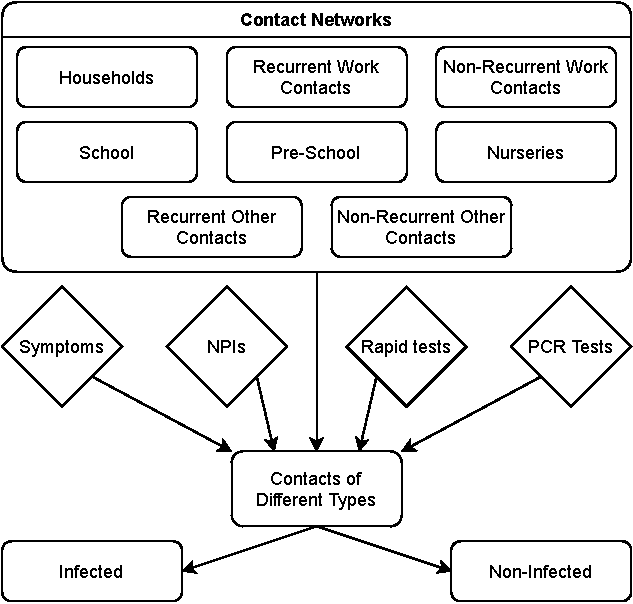
\includegraphics[width=\textwidth]{../figures/model-graph-top-left}
        \caption{{\small Model description}}
        \label{fig:model_graph}
    \end{subfigure}
    \hfill
    \begin{subfigure}[b]{0.475\textwidth}
        \centering
        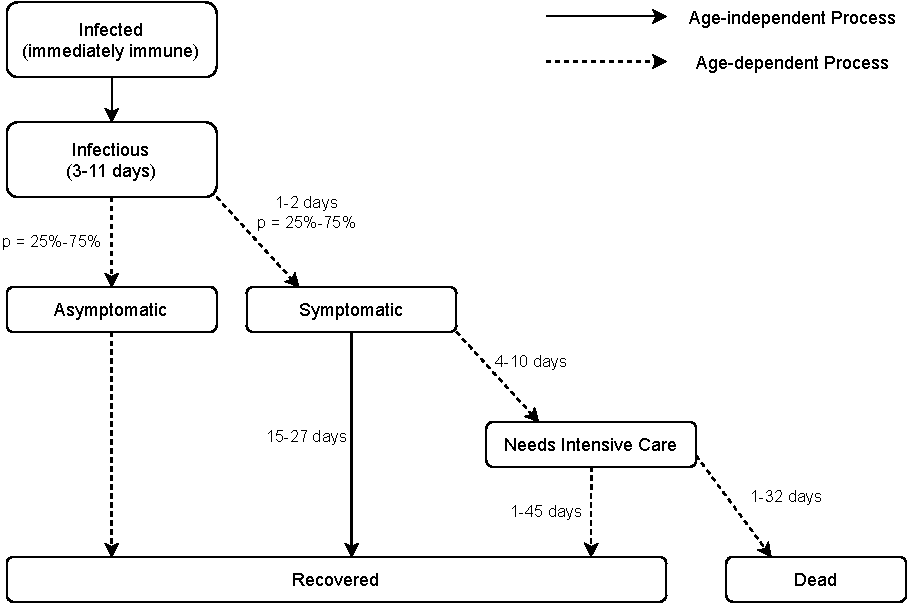
\includegraphics[width=\textwidth]{../figures/model-graph-top-right}
        \caption{Disease progression}
        \label{fig:disease_progression}
    \end{subfigure}

    \vskip3ex

    \begin{subfigure}[b]{0.475\textwidth}
        \centering

        PCR tests: quarantine (?)

        Antigen tests: subsequent PCR tests, quarantine, work/school

        Effects on other people (tracing)

        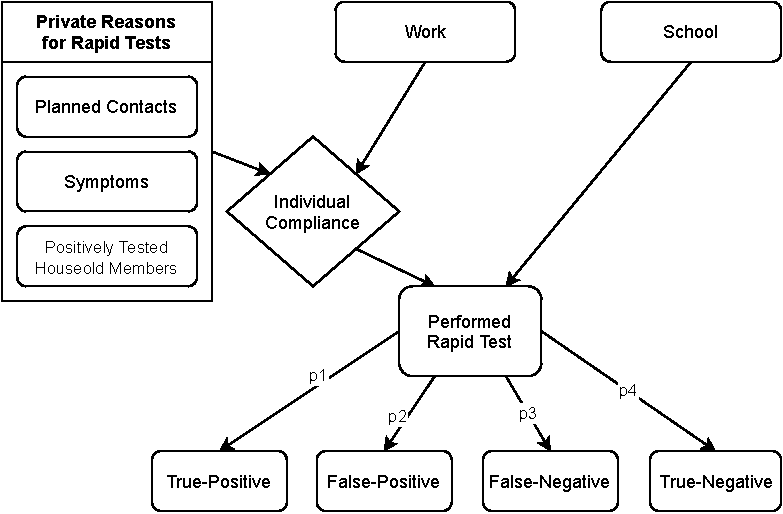
\includegraphics[width=\textwidth]{../figures/model-graph-bottom-left}
        \caption{{\small PCR and antigen tests}}
        \label{fig:pcr_antigen_tests}
    \end{subfigure}
    \begin{subfigure}[b]{0.475\textwidth}
        \centering

        Model for detected/undetected cases

        % 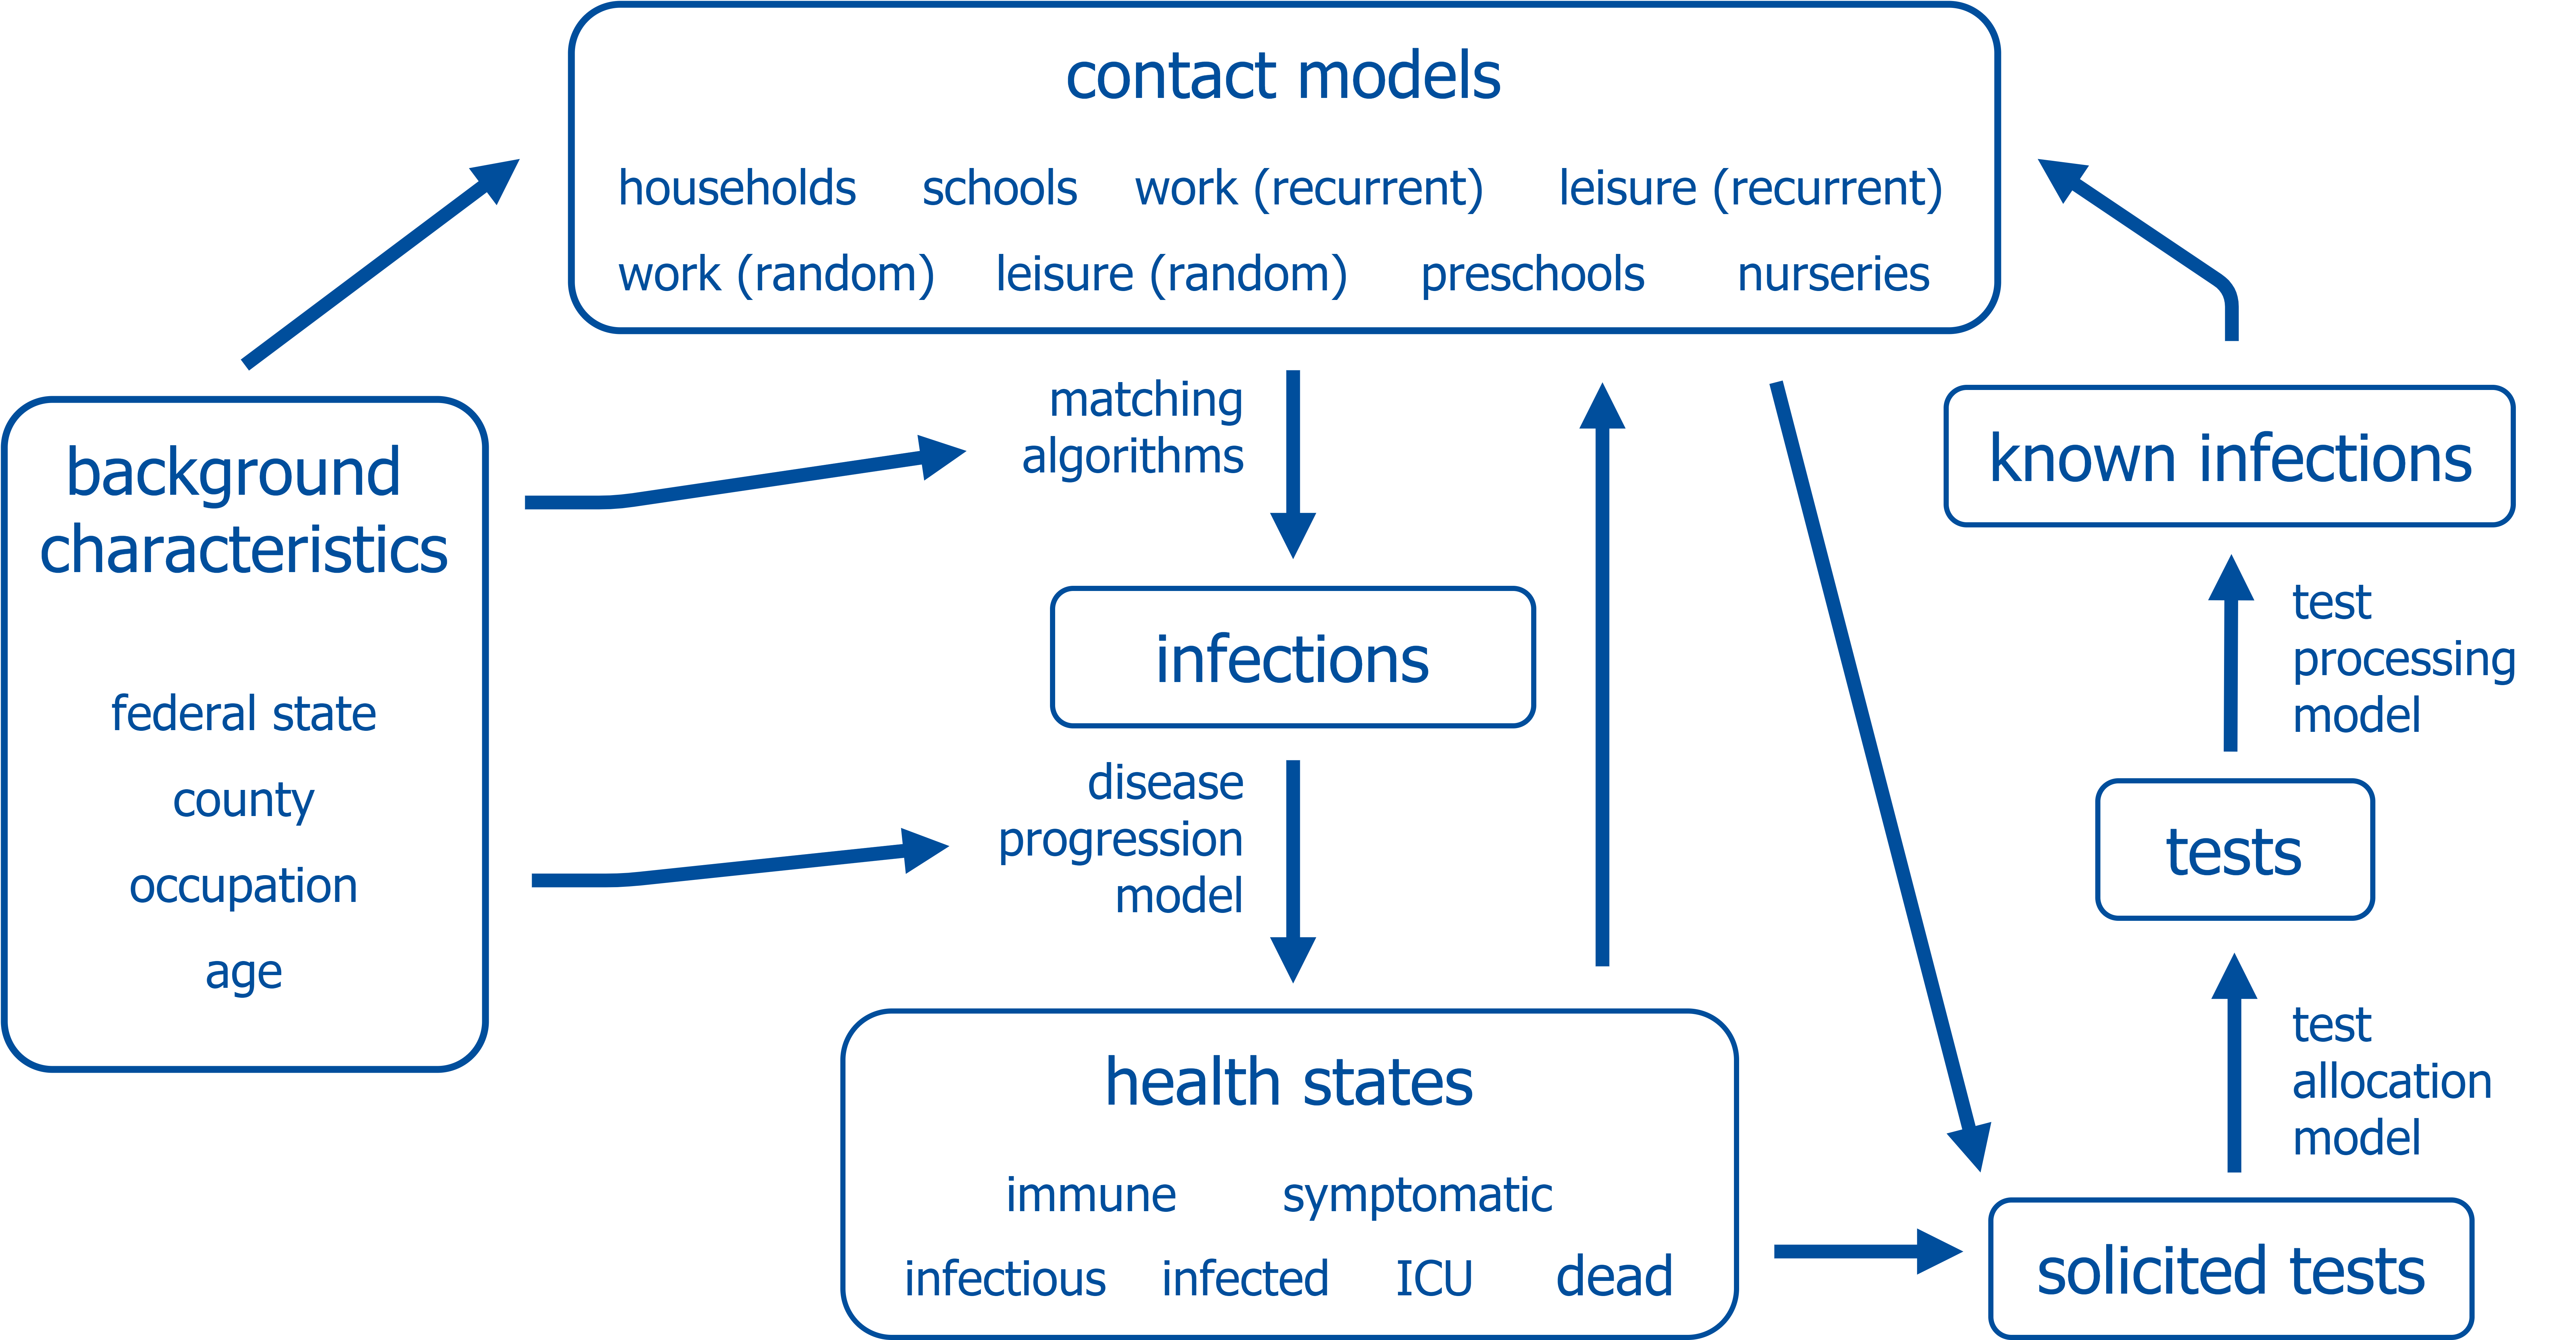
\includegraphics[width=\textwidth]{../figures/model_detailed.png}
        \caption{{\small Model for translating simulated number to officially recorded cases}}
        \label{fig:model_for_official_cases}
    \end{subfigure}

    \caption{Model description}
\end{figure}


Susceptibility to contracting CoViD-19 is dependent on age and so is the progression of the disease. We differentiate between an inital period of infection without being infectious or showing symptoms, being infectious (presymptomatic or asymptomatic), showing symptoms, requiring intensive care, and recovery or death. The probabilities of transitioning between these states depend on age; their duration is random within intervals calibrated to medical literature.\comment[id=HM]{Cite}. Conditional on the type of contact, infectiousness independent of ages.\comment[id=HM]{Cite current Drosten paper}

The model includes several other features, which are crucial to describe the evolution of the pandemic in 2020-2021. New virus strains with different profiles regarding infectiousness and disease progress can be introduced. With a probability calibrated to XXX\comment[id=HM]{Klara, please add citatiion}, vaccinated agents become immune and they do not transmit the virus. While vaccines are rolled out, priority may depend on age and occupation. Agents may demand two types of tests as described in Figure~\ref{fig:pcr_antigen_tests}. First, polymerase chain reaction (PCR) tests directly reveal whether an individual is infected or not. PCR tests require some time to be processed and there are always aggregate capacity constraints. Second, rapid antigen tests yield immediate results. Specificity and sensitivity of these tests is set according to the XXX data.\comment[id=HM]{subsequent PCR tests, quarantine, work/school}. Demand for rapid tests will depend on policy, e.g., prices, testing requirements before work, attending school, or visiting restaurants and shops.


Identification

Modelling a population of agents according to actual demographic characterists means that we can use a wide array of data to estimate the model parameters. Mobility data is used to inform reductions in work and social contacts.\comment[id=HM]{check} School and daycare policies can be incorporated directly from official directives. Infection rates by age and geographical region are matched to officially recorded numbers, so is the prevalence of virus strains. In order to translate simulated cases in our model to officially recorded cases, we use the model depicted in Figure~\ref{fig:model_for_official_cases}. 

Simulated data have very similar structure to data that is used for regression analyses. Can use as further plausbility check.

\paragraph{Example: Germany}
\begin{itemize}
    \item Good first response, relatively lax (no curfew, few business closures, ... )
    \item Then relaxed over the summer at low incidence rates
    \item Cross-country mobility planted the seeds for fall wave
    \item We start our analysis at this point because modelling undetected cases would require a very different approach than in spting
\end{itemize}


\begin{figure}[!tp]
    \centering

    \begin{subfigure}[b]{0.475\textwidth}
        \centering
        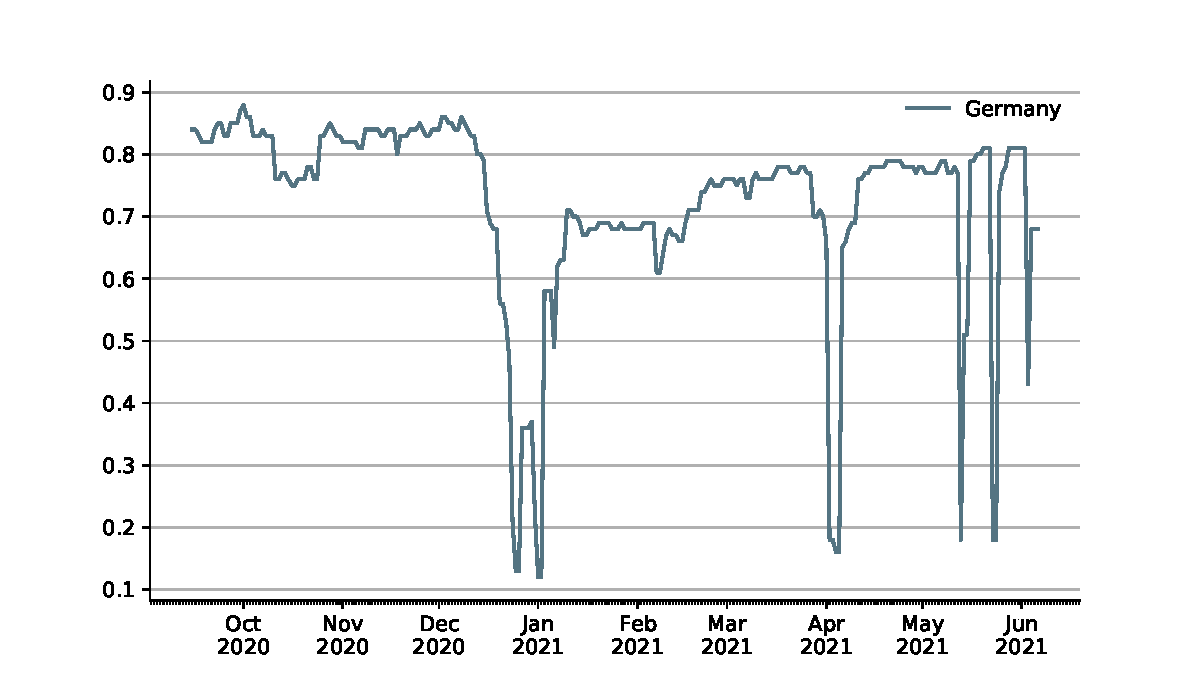
\includegraphics[width=\textwidth]{../figures/results/figures/data/work_multiplier_since_sep}

        Stringency index + multipliers

        Contact reduction $\times$ hygiene multiplier for different types of contacts 
        
        potentially $\times$ seasonality

        else put seasonality separately
        \begin{itemize}
            \item Work
            \item School
            \item Other
        \end{itemize}

        \caption{{\small Contact reductions}}
        \label{fig:stringency_index}
    \end{subfigure}
    \hfill
    \begin{subfigure}[b]{0.475\textwidth}
        \centering

        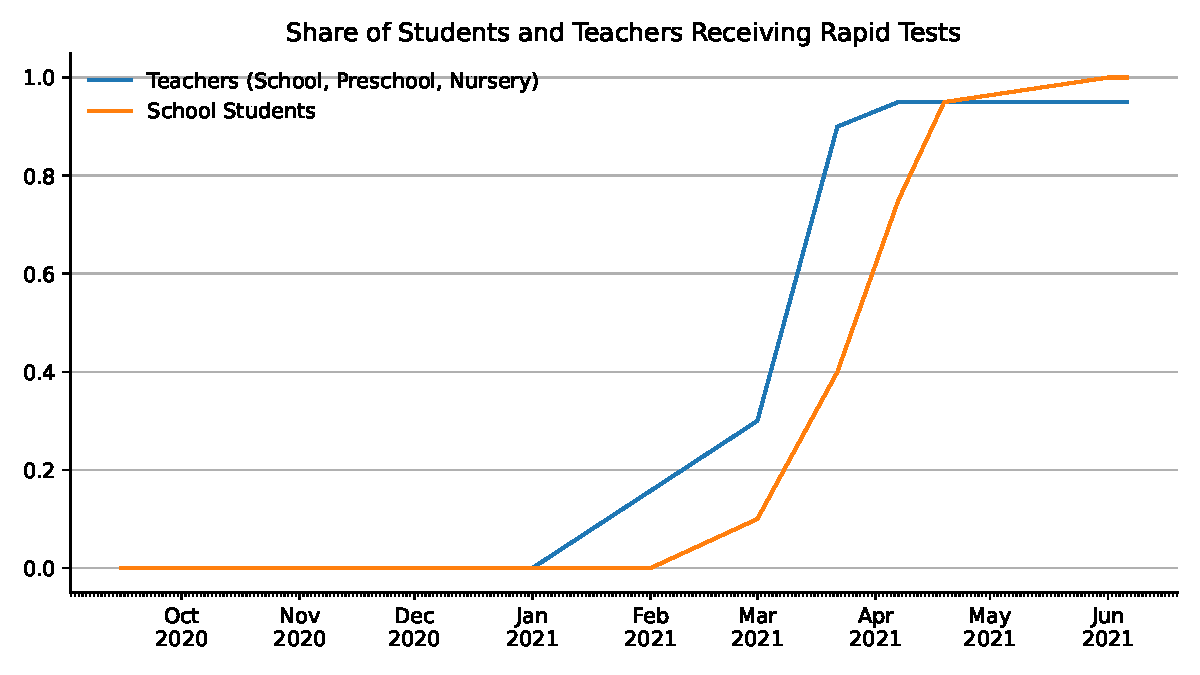
\includegraphics[width=\textwidth]{../figures/results/figures/data/testing/share_of_educ_participants_with_rapid_test}

        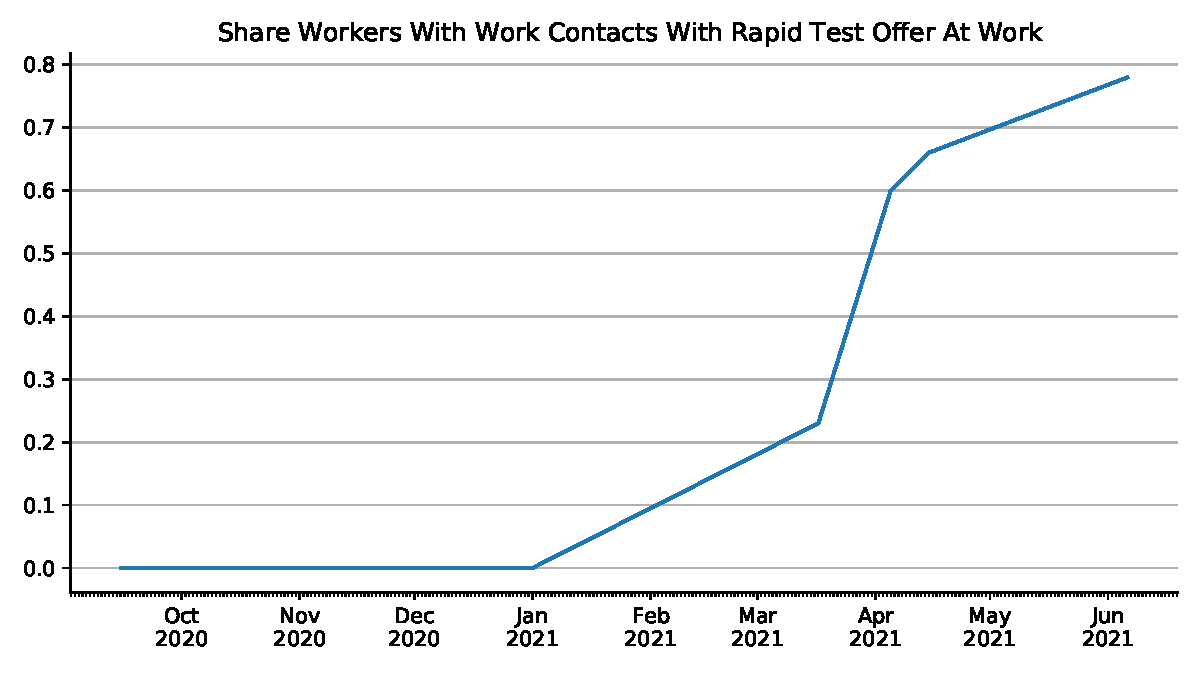
\includegraphics[width=\textwidth]{../figures/results/figures/data/testing/share_of_workers_with_rapid_test_offer_at_work}
        % fraction of workers must be multiplied with 0.6 because only that many actually
        % accept the offer

        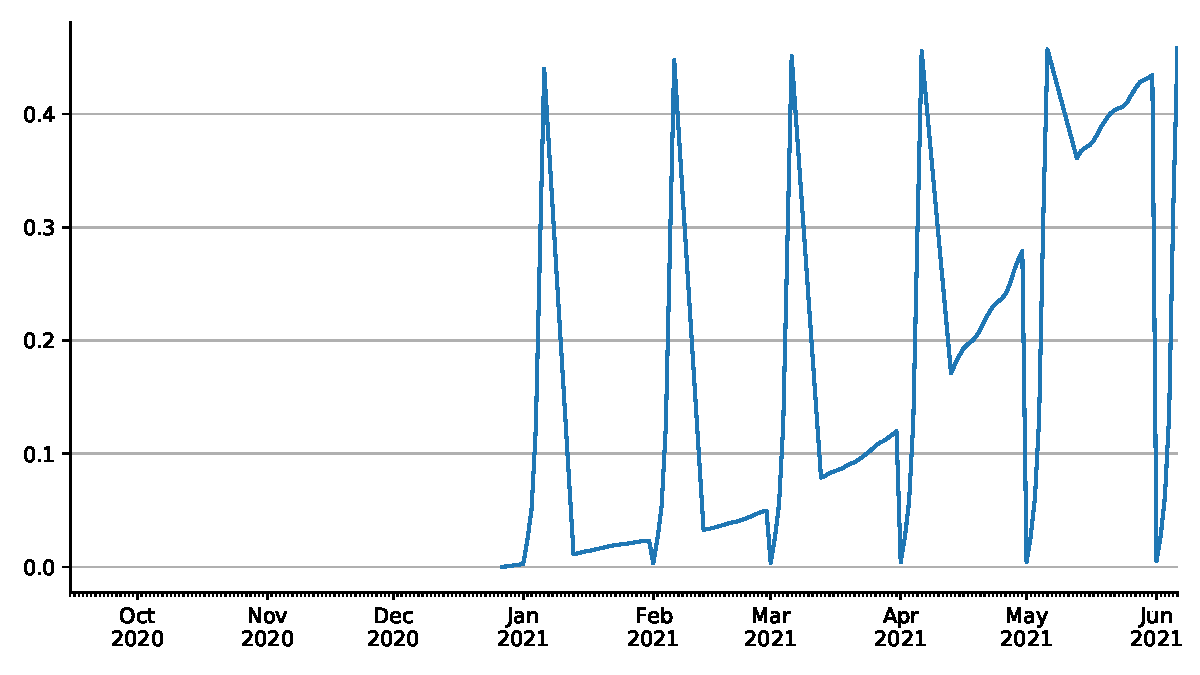
\includegraphics[width=\textwidth]{../figures/results/figures/data/share_of_individuals_with_first_vaccine}

        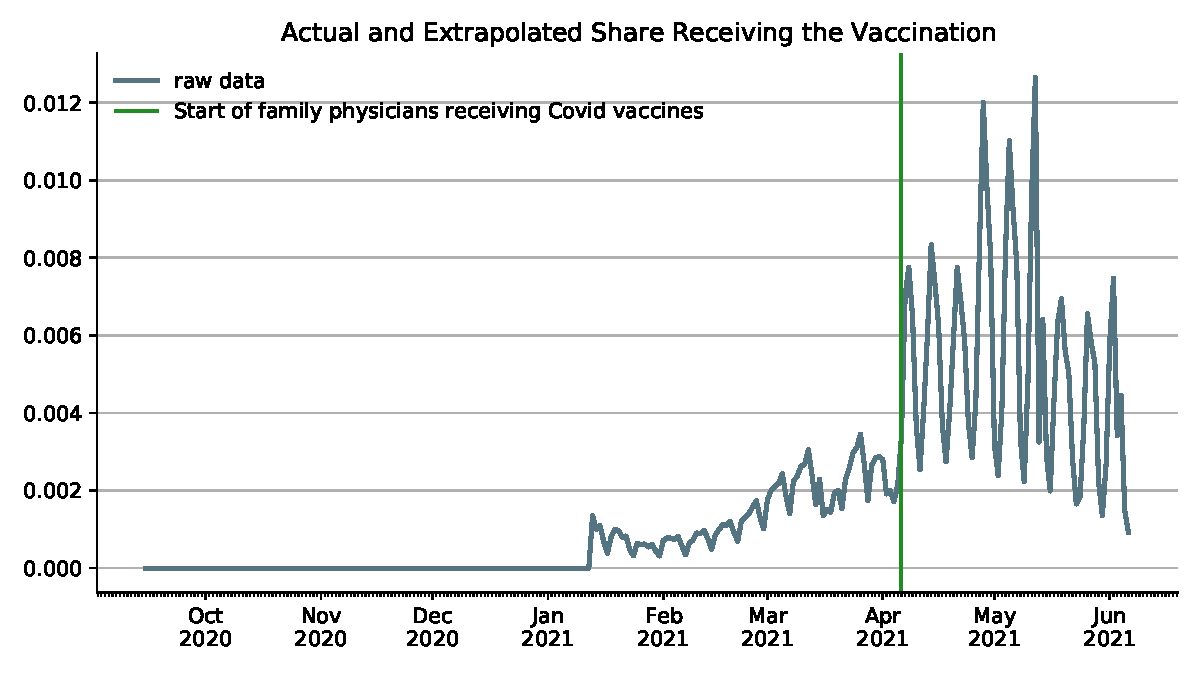
\includegraphics[width=\textwidth]{../figures/results/figures/data/share_receiving_vaccination_per_day}

        Number of PCR tests

        \vskip2ex

        \caption{{\small Tests and vaccinations}}
        \label{fig:pcr_antigen_tests_vaccinations}
    \end{subfigure}
    \vskip3ex
    
    \begin{subfigure}[b]{0.475\textwidth}
        \centering
        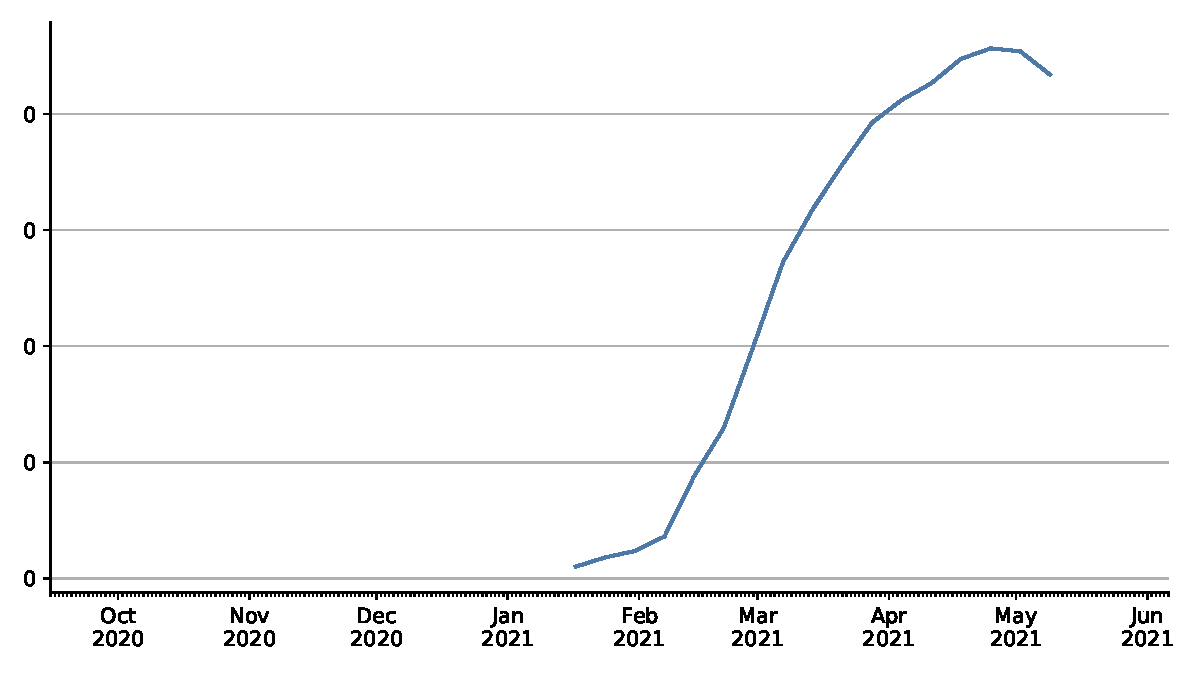
\includegraphics[width=\textwidth]{../figures/results/figures/data/share_of_b117_acc_to_rki}

        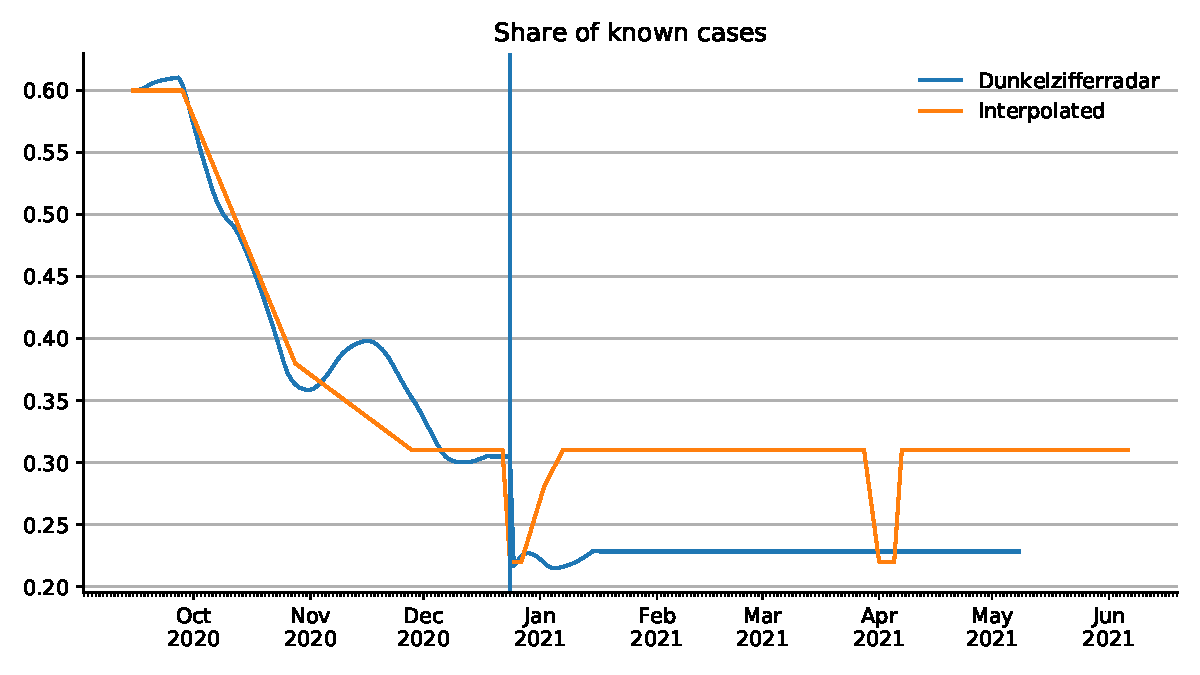
\includegraphics[width=\textwidth]{../figures/results/figures/data/testing/assumed_overall_share_known_cases}

        \vskip2ex

        \caption{Share of known cases and fraction of B.1.1.7 strain}
        \label{fig:share_known_cases_b117}
    \end{subfigure}
    \begin{subfigure}[b]{0.475\textwidth}
        \centering

        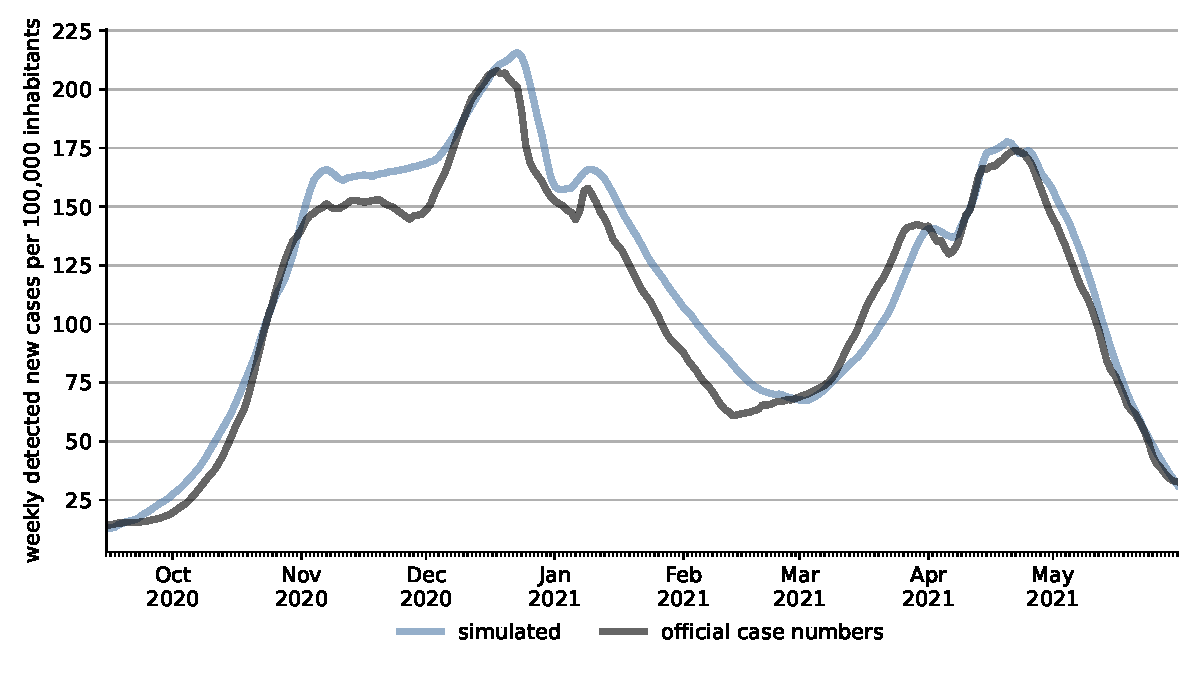
\includegraphics[width=\textwidth]{../figures/results/figures/scenario_comparisons/combined_fit/full_new_known_case}
        \caption{{\small Recorded cases: Empirical and simulated}}
        \label{fig:aggregated_fit}
    \end{subfigure}

    \caption{Drivers of the pandemic and model fit, September 2020 to May 2021}
    \label{fig:pandemic_drivers_model_fit}

    Note: All aggregates; See S.XXX for statistics by age group and by geographical region.

\end{figure}



\begin{figure}[!tp]
    \centering

    \begin{subfigure}[b]{0.475\textwidth}
        \centering
        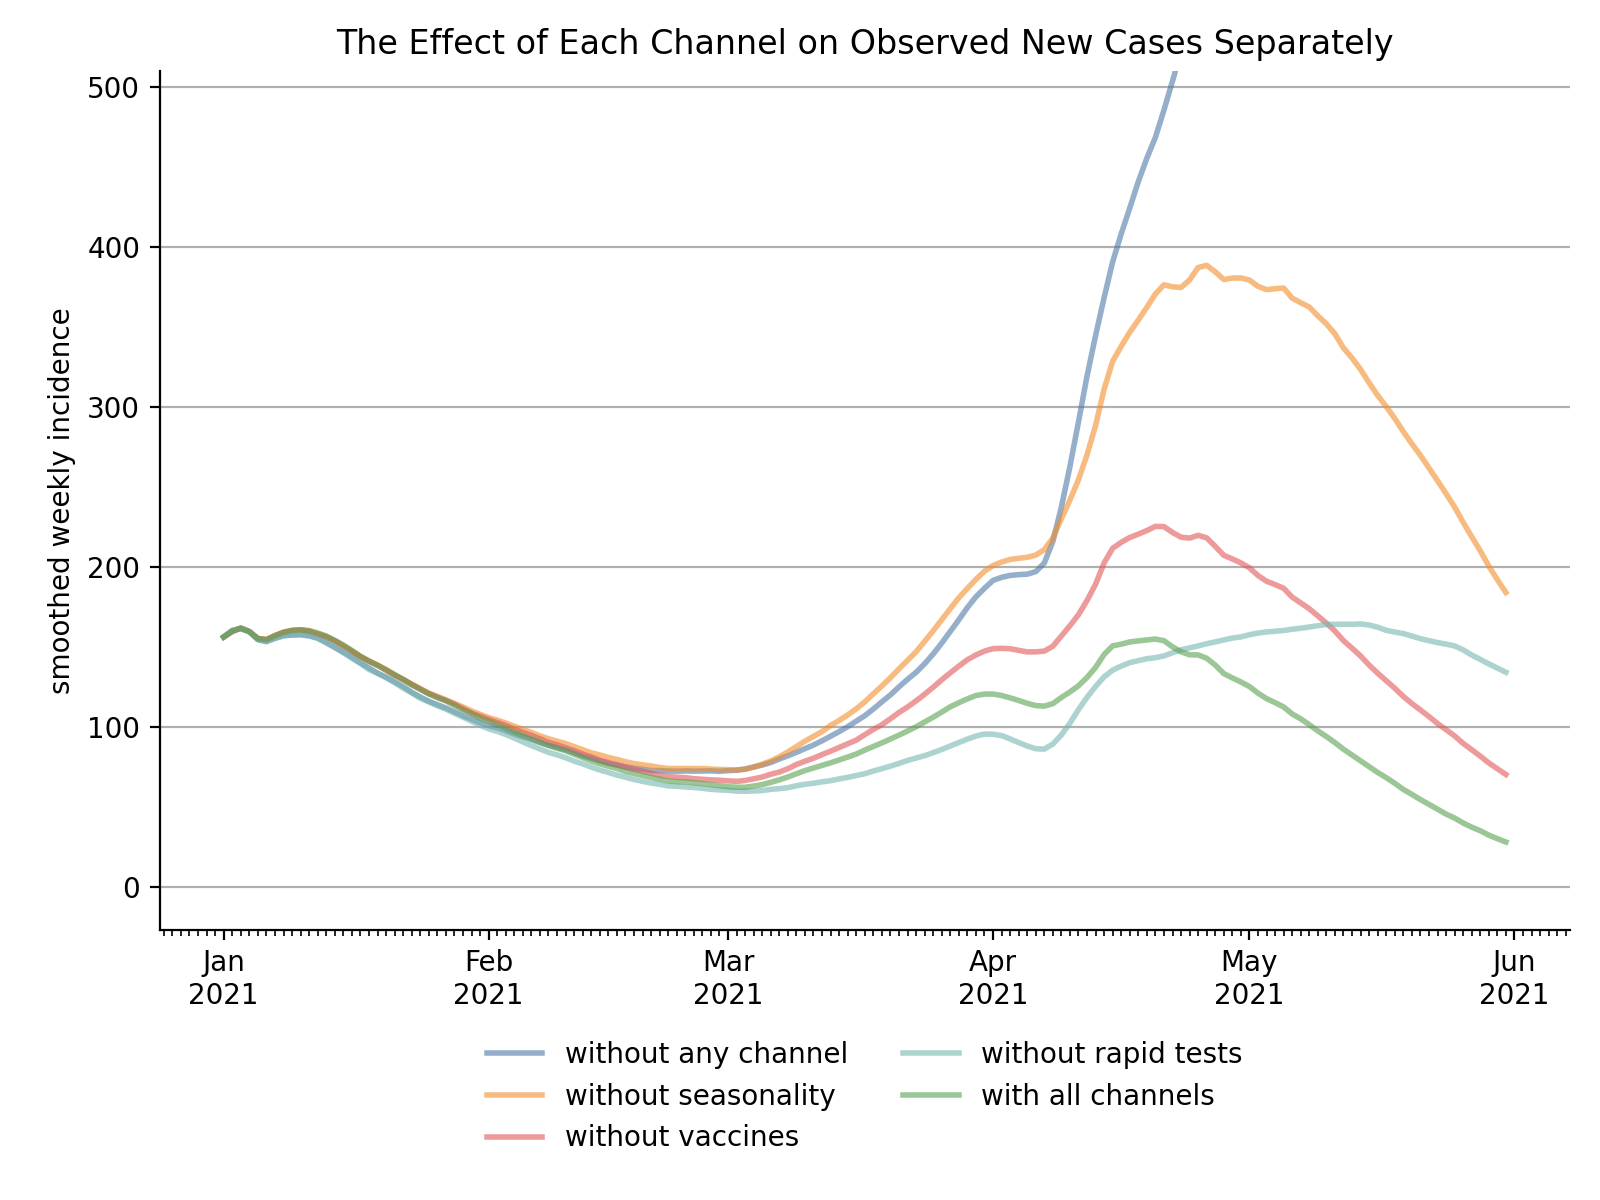
\includegraphics[width=\textwidth]{../figures/results/figures/scenario_comparisons/one_off_and_combined/full_new_known_case_cropped}
        \caption{{\small Recorded cases: 2021 scenarios}}
        \label{fig:full_new_known_case_cropped}
    \end{subfigure}
    \hfill
    \begin{subfigure}[b]{0.475\textwidth}
        \centering

        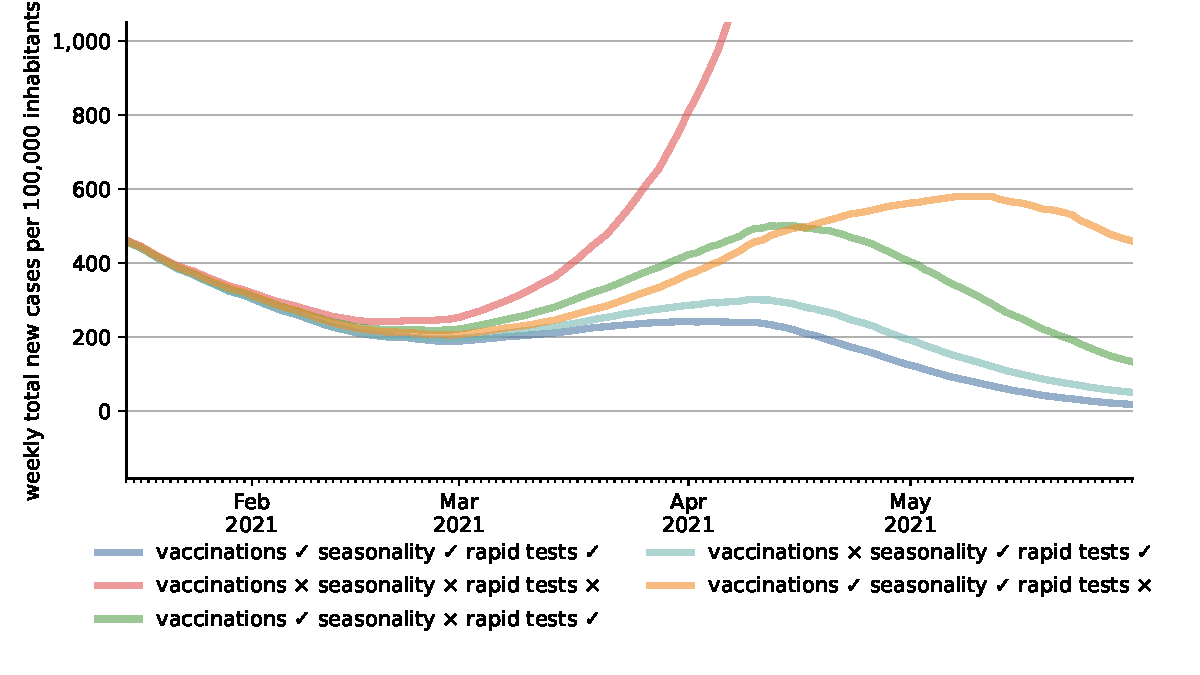
\includegraphics[width=\textwidth]{../figures/results/figures/scenario_comparisons/one_off_and_combined/full_newly_infected_cropped}
        \caption{{\small Total cases: 2021 scenarios}}
        \label{fig:full_newly_infected_cropped}
    \end{subfigure}
    \vskip3ex
    
    \begin{subfigure}[b]{0.475\textwidth}
        \centering
        % 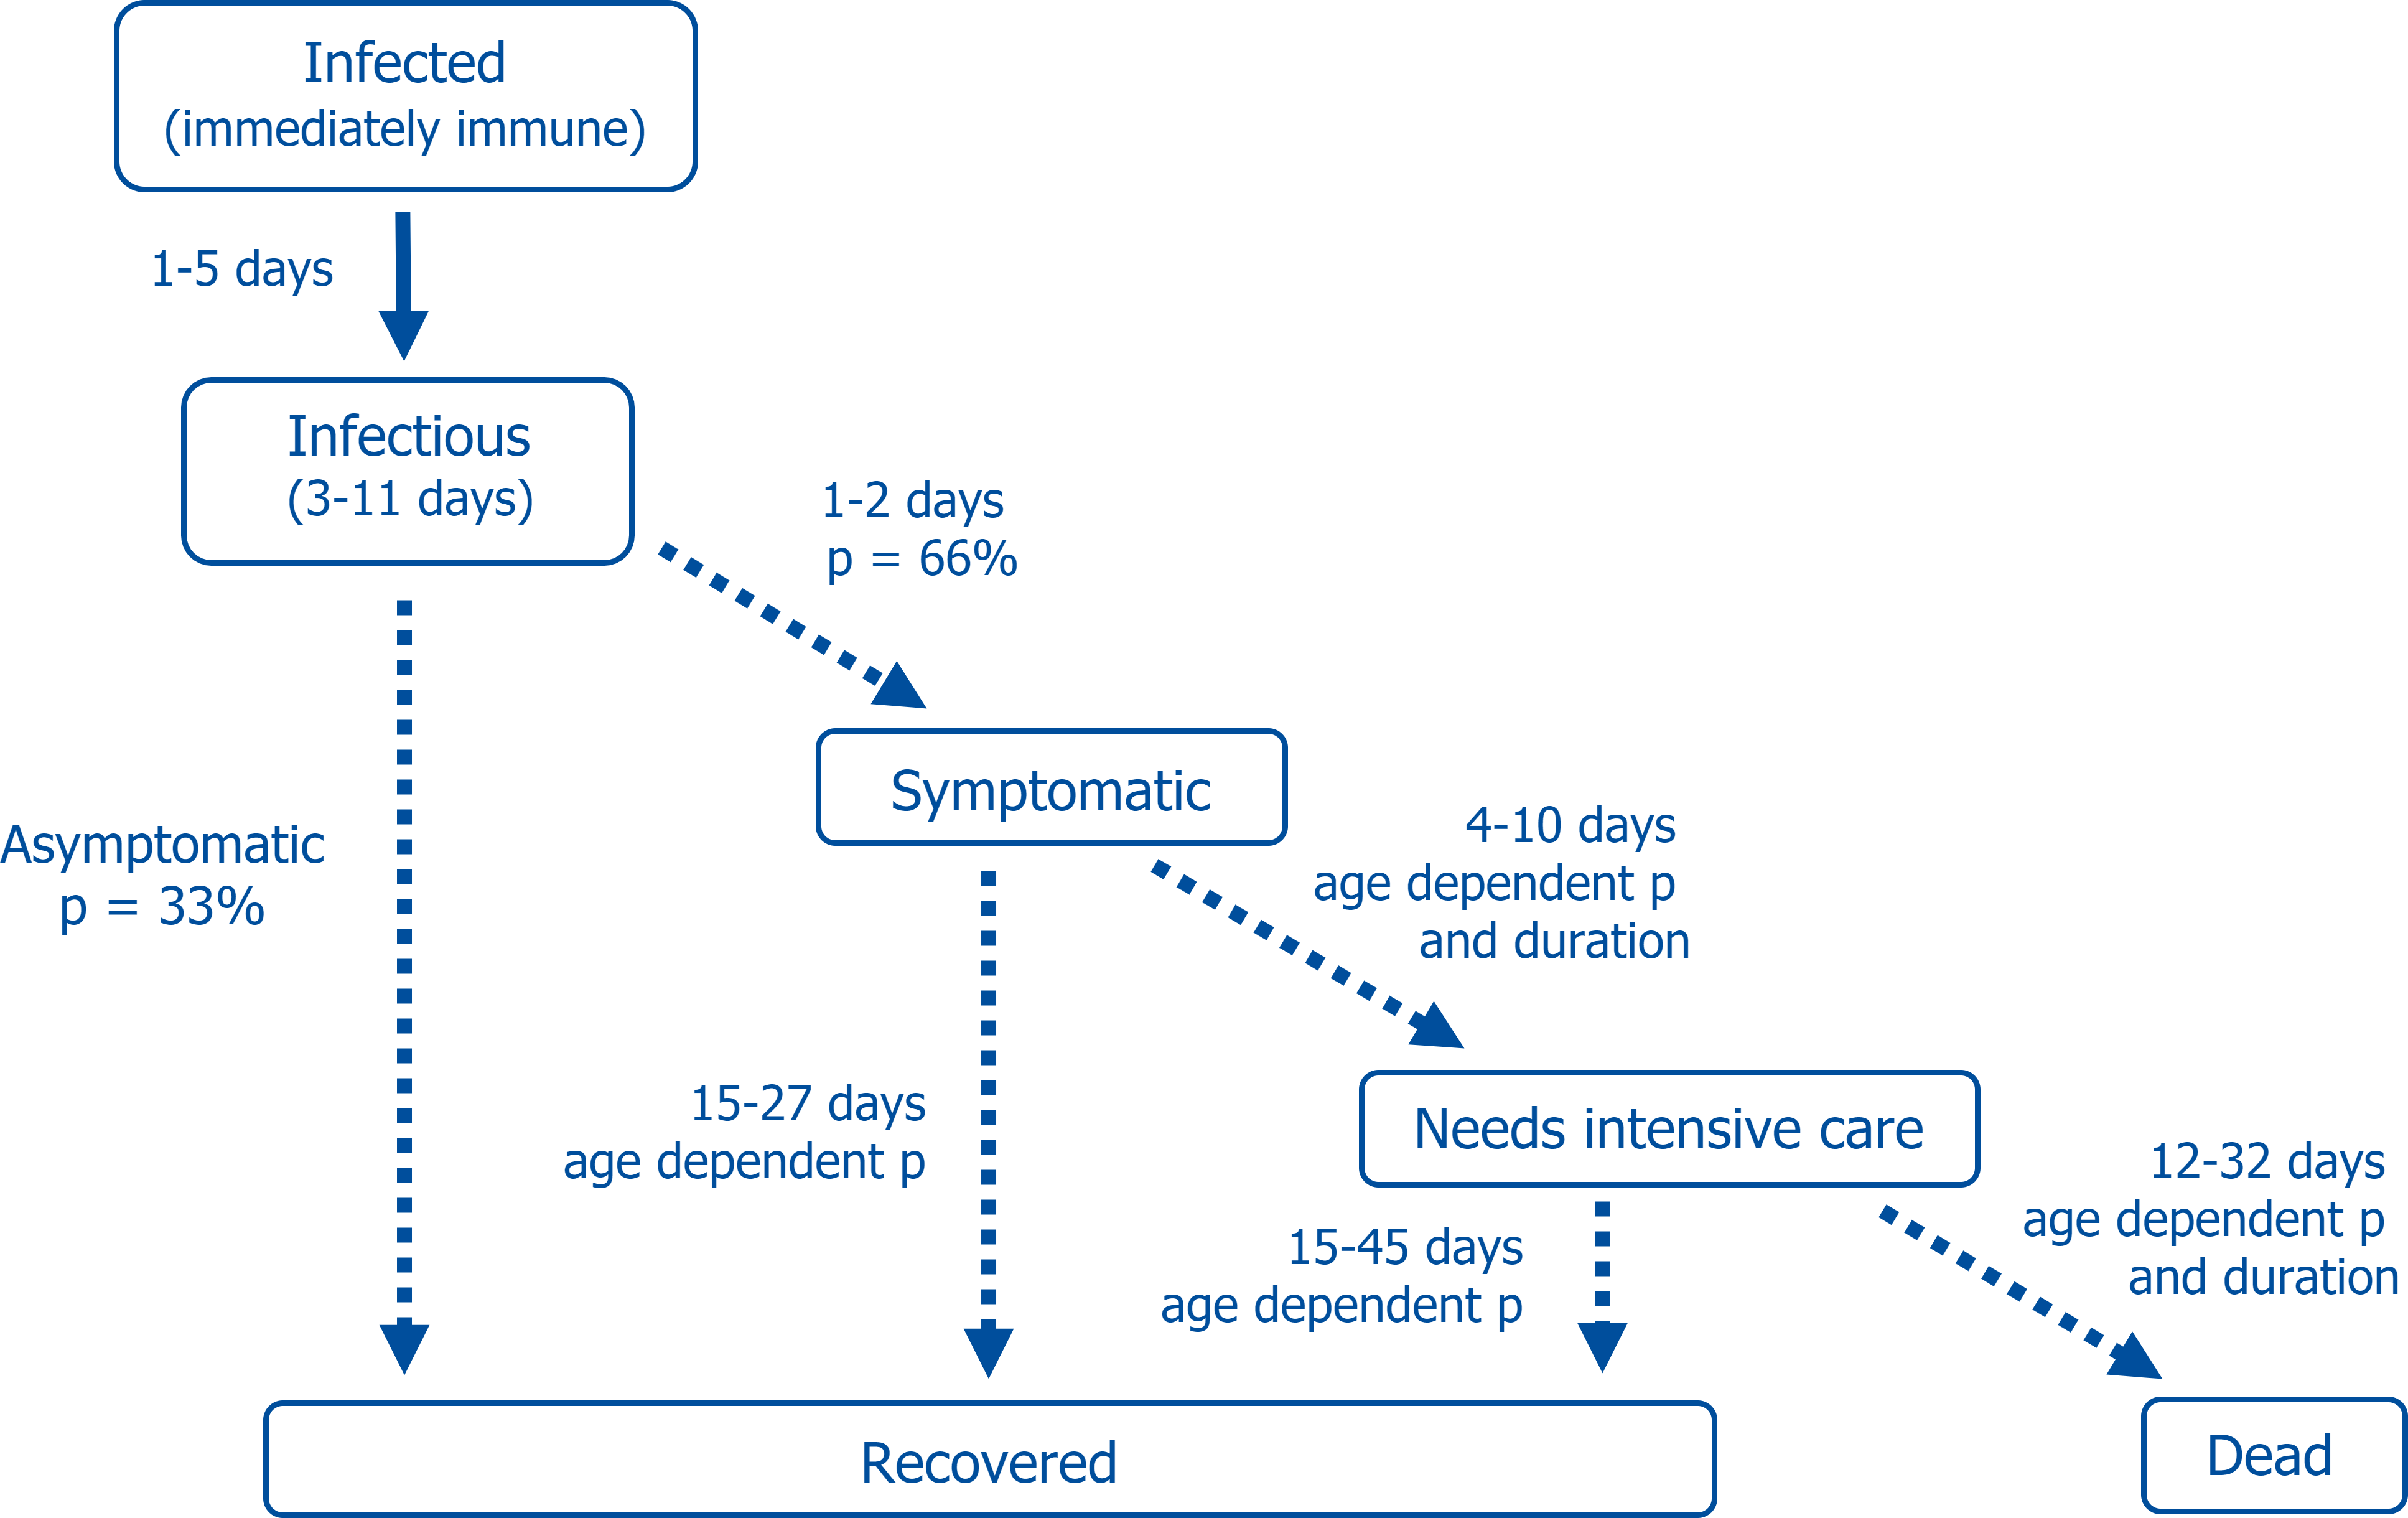
\includegraphics[width=\textwidth]{../figures/disease_progression.png}

        Shapley values

        \vskip2ex

        \caption{Decomposition of effects for Figure~\ref{fig:full_newly_infected_cropped}}
        \label{fig:decompisition total cases}
    \end{subfigure}
    \begin{subfigure}[b]{0.475\textwidth}
        \centering

        % 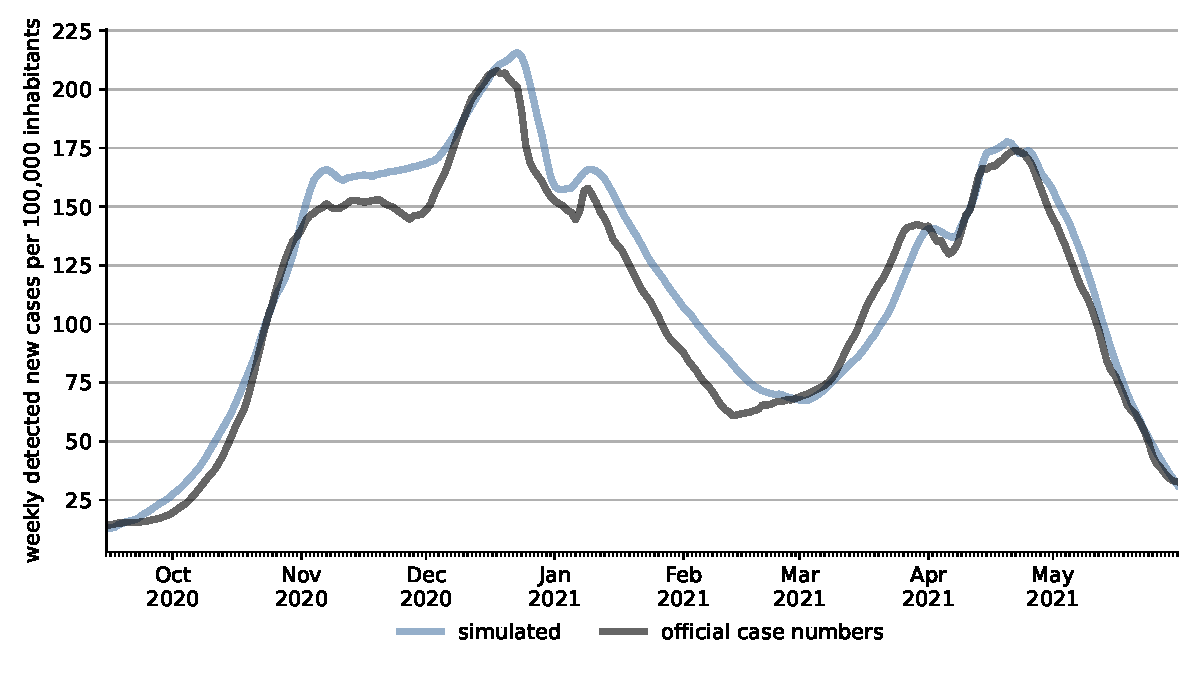
\includegraphics[width=\textwidth]{../figures/results/figures/scenario_comparisons/combined_fit/full_new_known_case}

        Effects of social structure (implicit tracing) / effects of different types of testing

        \vskip2ex

        \caption{{\small Effects of different types of testing}}
        \label{fig:decomposition_tests}
    \end{subfigure}

    \caption{The effect of different interventions on recorded and actual infections}
    \label{fig:interventions_broad}

    Note: All aggregates; See S.XXX for statistics by age group and by geographical region.

\end{figure}


\begin{figure}[!tp]
    \centering

    \begin{subfigure}[b]{0.475\textwidth}
        \centering
        % 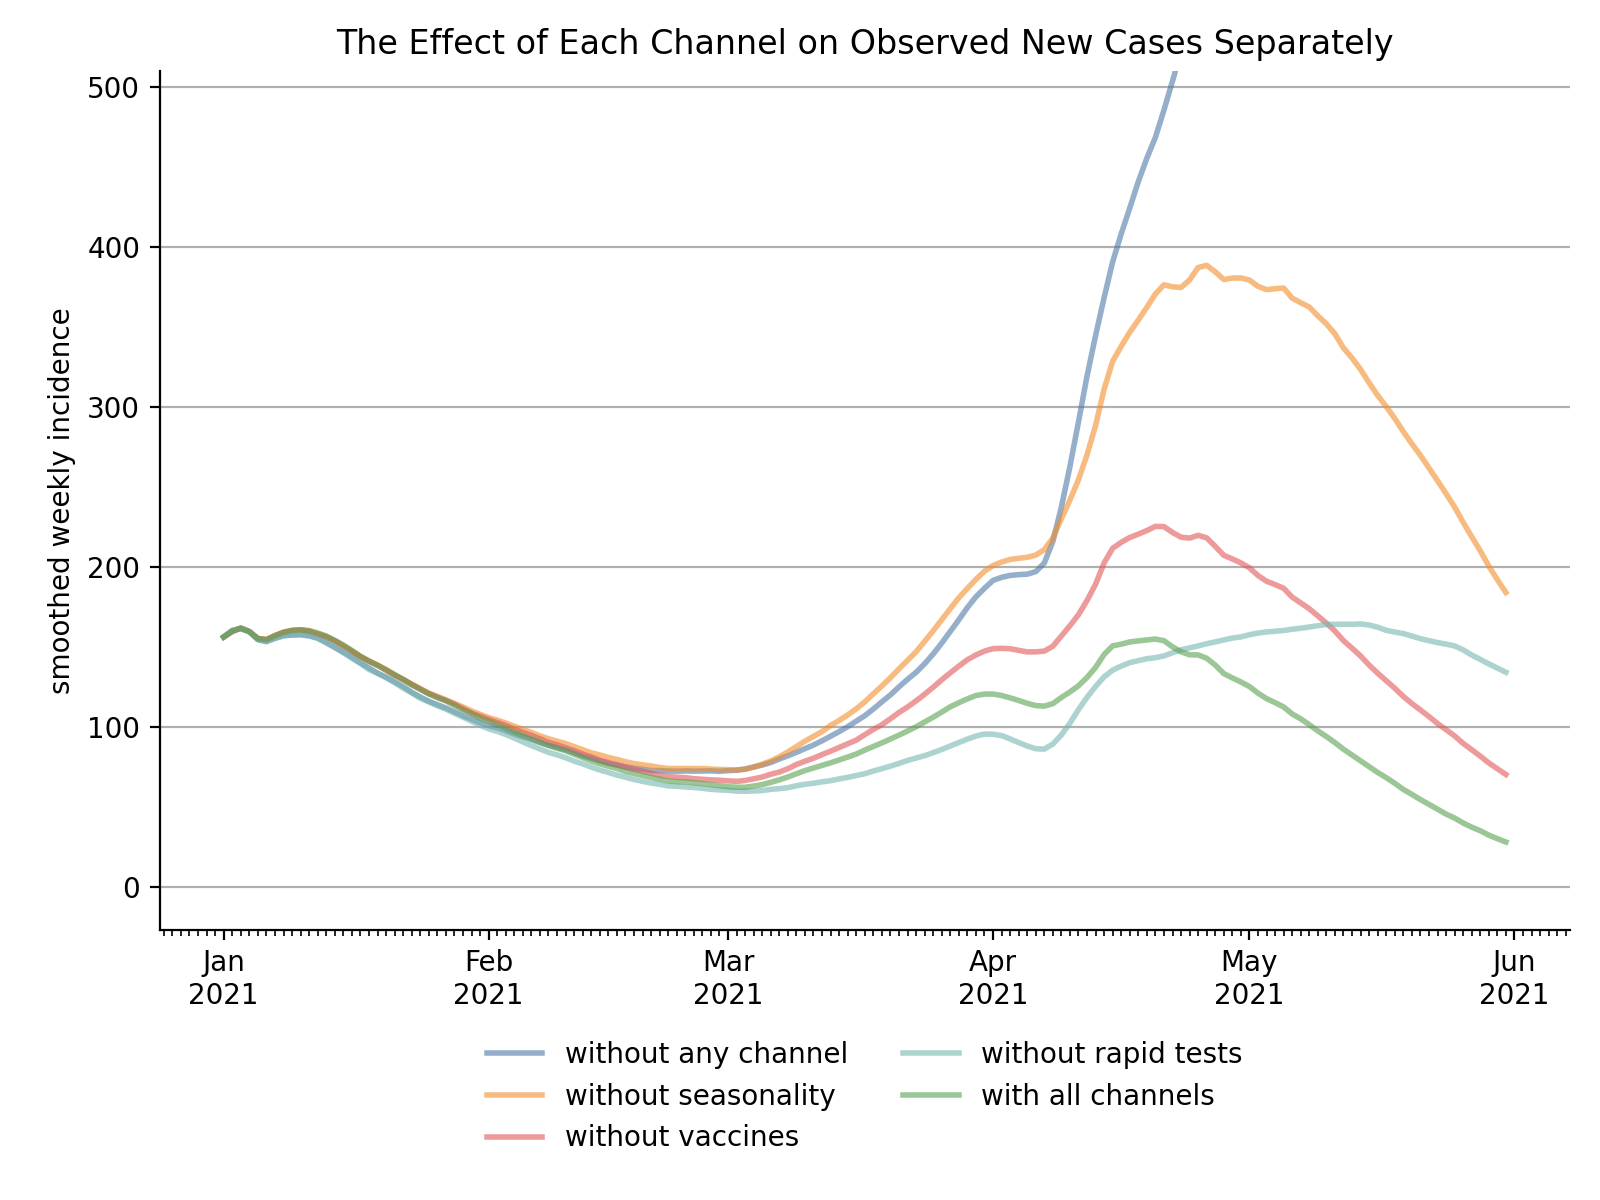
\includegraphics[width=\textwidth]{../figures/results/figures/scenario_comparisons/one_off_and_combined/full_new_known_case_cropped}
        \caption{{\small Effects of different schooling scenarios after Easter}}
        \label{fig:schooling_scenarios_easter}
    \end{subfigure}
    \hfill
    \begin{subfigure}[b]{0.475\textwidth}
        \centering

        % 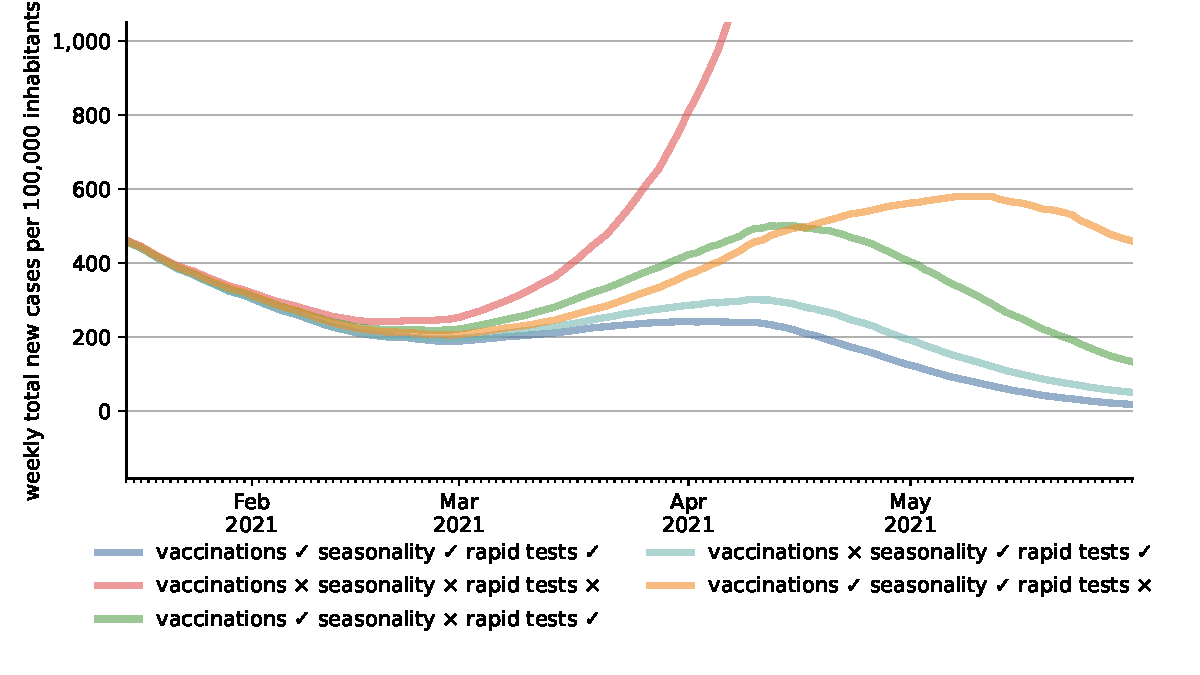
\includegraphics[width=\textwidth]{../figures/results/figures/scenario_comparisons/one_off_and_combined/full_newly_infected_cropped}
        \caption{{\small TBD}}
        \label{fig:to_be_determined}
    \end{subfigure}
    \vskip3ex    

    \caption{Schooling / maybe home office}
    \label{fig:interventions_school}

    Note: All aggregates; See S.XXX for statistics by age group and by geographical region.

\end{figure}



\paragraph{Points to mention}
\begin{itemize}
    \item If anything too optimistic regarding vaccinations
    \item Social structure / conditional block testing in families important (?)
    \item Trump-effect: More testing = more cases true for how long?
\end{itemize}

% Technical terms should be defined. 

% Symbols, abbreviations, and acronyms should be defined the first time they are used. 

% All tables and figures should be cited in numerical order.

% All data must be shown either in the main text or in the Supplementary Materials or must be available in an established database with accession details provided in the acknowledgements section.

% References to unpublished materials are not allowed to substantiate significant conclusions of the paper.


\section{Supplementary Material}

\begin{enumerate}
    \item Model
    \item Data
    \item Identification and Estimation
\end{enumerate}